\menudef{menu.help.manual}

The application's manual is available as either a \gls{pdf}
document, which can be viewed outside of the application, or as a
set of \gls{html} files which can be viewed within the application
via the \menu{help.manual} menu item. This will open the primary
help window (\sectionref{sec:primaryhelp}), but some dialog boxes
may also have a \btn{help} button that will open a secondary help
dialog (\sectionref{sec:secondaryhelp}).

\section{The Primary Help Window}
\label{sec:primaryhelp}

The main help frame has a panel that shows a page of the manual.  Links
in the page and the \gls{gui} navigation elements provide a way to
switch to a different page.  Note that \qt{page} in this context
refers to the file displayed in the help window, which typically
contains a section, and doesn't relate to the page numbers in the
\gls{pdf}.

There is a menu bar with items for navigation actions or adjusting
\gls{gui} settings. Some menu items are replicated as buttons in the
toolbar, which is split into different regions: navigation,
settings, and history. The forward, up and next navigation actions
can also be implemented by buttons in the lower navigation panel at
the bottom of the window.

\menudef*{menu.helpframe.navigation}

The \menu{helpframe.navigation} menu provides a way to move around
the document.
\Figureref{fig:navbuttons} shows the four navigation
buttons: \btn{helpframe.navigation.home} (go to the start of the manual), 
\btn{helpframe.navigation.previous} (go to the previous section), 
\btn{helpframe.navigation.up} (go to parent section), and 
\btn{helpframe.navigation.next} (go
to the next section).

\FloatFig
{fig:navbuttons}
{\includeimg
 [alt=
   {
     [\entrytooltip{menu.helpframe.navigation.home} Button]
     [\entrytooltip{menu.helpframe.navigation.previous} Button]
     [\entrytooltip{menu.helpframe.navigation.up} Button]
     [\entrytooltip{menu.helpframe.navigation.next} Button]
   }
 ]{images/navbuttons}%
}
[Navigation Buttons]{Navigation Buttons (Home, Previous, Up, Next)}

\menudef{menu.helpframe.navigation.home}

The \menu{helpframe.navigation.home} item, which is also available
as a button on the toolbar, will replace the current view with the
first page of the document.

\menudef{menu.helpframe.navigation.up}

The \menu{helpframe.navigation.up} item, which is also available
as a button on the toolbar, will replace the current view with the
parent page of the current hierarchical level. The item and button
will be disabled if there is no parent page. The parent page may
also be the previous page if the current page is the first in its
current hierarchical level.

\menudef{menu.helpframe.navigation.previous}

The \menu{helpframe.navigation.previous} item, which is also available as
a button on the toolbar, will replace the current view with the
previous page. The item and button will be disabled if there is no
previous page. (That is, if the current page is the first
page of the document.)

\menudef{menu.helpframe.navigation.next}

The \menu{helpframe.navigation.next} item, which is also available as
a button on the toolbar, will replace the current view with the
next page. The item and button will be disabled if there is no
next page. (That is, if the current page is the last
page of the document.)

\Figureref{fig:search+index} shows the search and index buttons.

\FloatFig
{fig:search+index}
{\includeimg
 [alt=
   {
     [\entrytooltip{menu.helpframe.navigation.search} Button]
     [\entrytooltip{menu.helpframe.navigation.index} Button]
   }
 ]{images/search+index}%
}
{Search and Index Buttons}

\menudef{menu.helpframe.navigation.search}

The \menu{helpframe.navigation.search} item, which is also available
as a button on the toolbar, will open the
\dialog{help.navigation.search} window (see
\figureref{fig:searchframe}), from which you can search the document
for a keyword. If any matches are found, the title of the relevant
page is shown as a hyperlink, which links to the start of the page.
The title is followed by a block of text where the search term was
found (which will be highlighted). Clicking on the block of text
should scroll to a nearby location in the relevant page.

\FloatFig
{fig:searchframe}
{\includeimg
 [alt=
   {image of search window showing search term highlighted in a paragraph}
 ]{images/searchframe}%
}
{Search Window}

\menudef{menu.helpframe.navigation.index}

The \menu{helpframe.navigation.index} item, which is also available
as a button on the toolbar, will open the index page in a separate
window (see \figureref{fig:indexframe}). You can also open the same
page in the help window at the end of the document. The index window
provides a way of navigating the document without having to keep
returning to the index page. Additionally, the index window has a
split page with links on the left to scroll the page to a letter
group.

\FloatFig
{fig:indexframe}
{\includeimg
 [alt=
   {image of index window showing part of the document index}
 ]{images/indexframe}%
}
{Index Window}

\Figureref{fig:historybuttons} shows the history buttons.
Note that the forward button is greyed (disabled) because the
currently viewed page is at the end of the history list, so it's not
possible to go forward.

\begin{figure}
\centering
\includeimg
 [alt=
  {[\entrytooltip{menu.helpframe.navigation.history} Button]
   [\entrytooltip{menu.helpframe.navigation.historyback} Button]
   [\entrytooltip{menu.helpframe.navigation.historyforward} Button]
  }
 ]
 {images/historybuttons-annote}

\caption{History Buttons}
\label{fig:historybuttons}
\end{figure}

\menudef{menu.helpframe.navigation.history}

The \menu{helpframe.navigation.history} menu item, which is also
available as a button on the toolbar, opens the
\dialog{help.navigation.history} window,
(see \figureref{fig:historywindow}).

The current page has the title shown in bold and is preceded by
the symbol \gls{symbol.help.navigation.history.pointer}.
Select the required page and click on the
\gls{help.navigation.history.go} button.

\begin{figure}
\centering
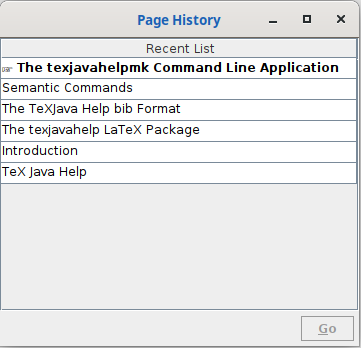
\includegraphics{images/historyframe}

\caption{The Page History Window}
\label{fig:historywindow}
\end{figure}

\menudef{menu.helpframe.navigation.historyback}

The \menu{menu.helpframe.navigation.historyback} menu item, which is
also available as a button on the toolbar, will replace the current
view with the previously viewed page from this history list. The
item and button will be disabled if there is no previously viewed
page. 

\menudef{menu.helpframe.navigation.historyforward}

The \menu{menu.helpframe.navigation.historyforward} menu item, which is
also available as a button on the toolbar, will replace the current view with the
next page in the history list. The item and button will be disabled if the
currently viewed page is at the end of the history list. 

\section{Secondary Help Window}
\label{sec:secondaryhelp}

The secondary help windows are more minimalist and will only show
the relevant page or set of pages that are applicable to the context
that was used to open the secondary help window. The search, history
and index items are unavailable. If only one page is applicable,
there won't be a navigation tree, otherwise the navigation tree will
only show the applicable pages.

